% ID = 35
%%%%%%%%%%%%%%%%%%%%%%% file template.tex %%%%%%%%%%%%%%%%%%%%%%%%%
%
% This is a general template file for the LaTeX package SVJour3
% for Springer journals.          Springer Heidelberg 2010/09/16
%
% Copy it to a new file with a new name and use it as the basis
% for your article. Delete % signs as needed.
%
% This template includes a few options for different layouts and
% content for various journals. Please consult a previous issue of
% your journal as needed.
%
%%%%%%%%%%%%%%%%%%%%%%%%%%%%%%%%%%%%%%%%%%%%%%%%%%%%%%%%%%%%%%%%%%%
%
% First comes an example EPS file -- just ignore it and
% proceed on the \documentclass line
% your LaTeX will extract the file if required
\begin{filecontents*}{example.eps}
%!PS-Adobe-3.0 EPSF-3.0
%%BoundingBox: 19 19 221 221
%%CreationDate: Mon Sep 29 1997
%%Creator: programmed by hand (JK)
%%EndComments
gsave
newpath
  20 20 moveto
  20 220 lineto
  220 220 lineto
  220 20 lineto
closepath
2 setlinewidth
gsave
  .4 setgray fill
grestore
stroke
grestore
\end{filecontents*}
%
\RequirePackage{fix-cm}
%
%\documentclass{svjour3}                     % onecolumn (standard format)
%\documentclass[smallcondensed]{svjour3}     % onecolumn (ditto)
\documentclass[smallextended]{svjour3}       % onecolumn (second format)
%\documentclass[twocolumn]{svjour3}          % twocolumn
\usepackage[cp1250]{inputenc}
%\usepackage[polish]{babel}
%\usepackage{polski}
%\usepackage{graphicx}
%\usepackage{amsthm}
\usepackage{amsmath}
\usepackage{amsfonts} %potrzebne do \mathbb{S}
\usepackage{overpic} %napisy na obrazkach
\usepackage{color}
%\usepackage[table]{xcolor}
%\usepackage{colortbl}
\usepackage{hhline}
\usepackage{dcolumn}
\usepackage{longtable}
\usepackage{fancyhdr}
\usepackage{subfig}
\usepackage{wrapfig}
\usepackage{here}
%\usepackage{breqn}
\usepackage{booktabs}
\usepackage{ctable}
\usepackage{caption}
\usepackage{color}
\def\red#1{{\color{red}{#1}\color{black}}}
\pagestyle{fancy}
\fancyhf{}
% numery stron: lewa do lewego (marginesu), prawa do prawego
\fancyhead[LE,RO]{\textbf{\thepage}}
% prawa pagina: zawarto�� \rightmark do lewego, wewn�trznego (marginesu)
\fancyhead[LO]{\small\sffamily \nouppercase{\rightmark}}
% lewa pagina: zawarto�� \leftmark do prawego, wewn�trznego (marginesu)
\fancyhead[RE]{\small\sffamily \nouppercase{\leftmark}}
% kreski oddzielaj�ce paginy (g�rn� i doln�):
\renewcommand{\headrulewidth}{0.4pt}
\renewcommand{\footrulewidth}{0.0pt}
\newcommand{\otoprule}{\midrule
[\heavyrulewidth]}\newtheorem{tw}{Theorem}
%\newtheorem{lemma}{Lemma}[section]
\newtheorem{df}{Definition}
\newtheorem{rmk}{Remark}

\smartqed  % flush right qed marks, e.g. at end of proof
%
\usepackage{graphicx}
%\usepackage{geometry}
%\geometry{tmargin=5cm,bmargin=4cm,lmargin=3cm,rmargin=3cm}
% \usepackage{mathptmx}      % use Times fonts if available on your TeX system
%
% insert here the call for the packages your document requires
%\usepackage{latexsym}
% etc.
%
% please place your own definitions here and don't use \def but
% \newcommand{}{}
%
% Insert the name of "your journal" with
% \journalname{myjournal}
%
\begin{document}

\title{Unsupervised anomaly detection for conveyor temperature SCADA data%\thanks{Grants or other notes
%about the article that should go on the front page should be
%placed here. General acknowledgments should be placed at the end of the article.}
}
%\subtitle{Do you have a subtitle?\\ If so, write it here}

%\titlerunning{Short form of title}        % if too long for running head

\author{Jacek Wodecki$^1$ \and Pawe{\l} Stefaniak$^1$ \and \\ Marta Polak$^1$ \and Rados{\l}aw Zimroz$^1$}

%\authorrunning{Short form of author list} % if too long for running head

\institute{$^1$KGHM CUPRUM Ltd., R\&D, Sikorskiego 2-8, 53-659, Wroc{\l}aw, Poland      %  \\
}


\date{Received: date / Accepted: date}
% The correct dates will be entered by the editor
\maketitle
\begin{abstract}
Belt conveyor system is a crucial element of ore transport process in underground copper ore mine. Damage of single belt conveyor might cause stopping of huge part of underground transport network, especially when failure concerns the main haulage conveyor line. For that reason it is important to use SCADA monitoring system. The symptom of damage can be found in increasing temperature measured within the system. Unfortunately, operating belt conveyors can be considered as time-varying system and direct decision making using temperature value is difficult. Long-term analysis of time series enables to learn how to recognize alarming moment. Thus the removal of failure can be scheduled so as to minimize the losses in production. In this paper the clustering method was applied to the long-term observations of the temperature in order to gearbox fault detection. Moreover, the breaks in the activity of belt conveyors (no operation) caused by holidays will be determined. The clustering algorithm identifies also  the specific character of the work at the beginning and end of week. 
\keywords{clustering algorithms \and SCADA system \and belt conveyor system \and temperature measurements}
%\PACS{05.45.Tp \and 05.10.-a \and 05.10.Ln}
%\subclass{62-07 \and 62F10 \and 62F40}
\end{abstract}
\section{Introduction} 
Today extraction of deposit is reaching into increasingly deeper parts of rock mass what is closely related to much higher deterioration of mining conditions in context of environment, safety and reliability of machinery park. Currently underground mining industry demands in terms of assumed efficiency relate to ensure high reliability and availability of the machines. Conscious planning of repair works allows to achieve full integration of machine system in good condition during the operation. Such approach is closely connected with predictive maintenance (PdM) based on condition monitoring that should crowd out currently machine maintenance procedures in use in mining industry \cite{Blazej2016,Jonak2006,Stefaniak2012}.
In copper ore mine case, this is especially important for belt conveyor network where damage of one belt conveyor might cause stopping of huge part of underground transportation system as well as LHD machinery operation \cite{Stefaniak2012}. \par
In the literature the topic of the optimal control and efficiency of the belt conveyors system is widely investigated \cite{Bartelmus2014,Krol2016,Zhang2010}. In the process of belt conveyors exploitation, SCADA systems record a lot of data represented as physical variables to monitor technological processes, especially degree of utilization, operational load and technical condition of the machines during their operation. Long term analysis of this data is very important in terms of understanding nature of the degradation process \cite{Astolfi2014,Bongers2008,c5}. It can allow to identify any anomalies occurring in the context of well established general case of behavior. In  practical  application  in  industry, especially in mining, acquired data are difficult to interpret due to external disturbances (noise, missing values, etc.) and  the complexity  of  monitored  processes/systems. Temperature time series are varying in time and difficult to estimate in wider time window. It depends on many factors like: 
\begin{itemize}
\renewcommand{\labelitemi}{$\bullet$}
\item Conveyor technical condition,
\item Conveyor design features,
\item External load of conveyor,
\item Location and role in transportation system,
\item Engine operation mode,
\item Environment parameters \cite{Obuchowski,Sawicki}.
\end{itemize}
Definition of set of statistical parameters and selection of appropriate analytical model for further classification is expected to lead to extraction of diagnostic information which is undoubtedly necessary to support maintenance staff \cite{Kaufman,Stefaniak2015}. Early detection of damage might establish opportunities to determine repair moment in optimal time during planned standstill of given conveyor systems.

In this paper, a procedure for processing and analysis of temperature data from gearbox has been presented. The paper is organized as follows. Firstly, description of industrial acquisition process data and its pre-processing procedure will be shown. Next, we will move on to the proposed algorithm for clustering of multivariate data. At the end of the article, the context analysis of temperature data and identification of anomalies in operation process will be discussed.
\section{Real data acquisition and pre-processing procedures}
SCADA systems used in copper ore mine allow to collect the data concerning information about operational parameters of underground machines. Measurement of the specific physical variables helps in monitoring  of condition of the machines and preventing damages. In this paper we analyze temperature data acquired by commercial, multichannel low frequency data logger installed on the belt conveyor gearbox in copper ore mine.

Before starting any data analysis one should be sure that the data were acquired properly and were cleaned from the incorrect values, what allow to avoid the false conclusions of analysis. The pre-processing procedures are obligatory in case of temperature data from belt conveyor gearbox, where we applied two-step procedure: cleaning data and resampling \cite{Wodecki}.

First step of data pre-processing was to remove the outliers observations. In the recorded data there were clearly visible incorrect values, for example negative temperatures. Such observations are not possible in the underground mine reality, where temperature varies between $20^o$C and $90^o$C. Therefore the all outliers observations should be erase from the recording.

Another problem is the non-equal sampling of examined data. For memory saving, temperature data begin record while the difference between two consecutive observations is large enough, that means it is higher than predefined threshold. Although that algorithm minimizes the size of data, the observations are not equally sampled, what hinders the analysis. Due to that, we should focus on adequate resampling procedure. In \cite{Wodecki} authors proposed the linear interpolation procedure to fill the missing observations. In view of the relatively small changes in the temperature during the short period of time, the mentioned method is appropriate to this kind of data. For each missing data time point, two neighboring recorded temperatures were taken and next the first order polynomial were fitted to them. The missing observation is replaced by value of fitted curve in specific time point. The data after application of pre-processing procedures are shown in Fig. \ref{fig: L222_55_data}.
\begin{figure}[ht!]
\vspace{-10pt}
\centering
\includegraphics[width = 1\textwidth]{Wykresy/L222_55_data.png}
\caption{Real temperature data from belt conveyor gearbox after pre-processing.}
\label{fig: L222_55_data}
\vspace{-10pt}
\end{figure}
As one can see on the time series in Fig. \ref{fig: L222_55_data}, there are visible cyclic drops of the temperature. They are connected to breaks at work in underground mine. In that time the gearbox is cooled to the ambient temperature. That specific behavior allows to easily split the data into fragments corresponding to each week of the belt conveyor operation. Moreover one can notice that at $33$rd day of collected data the sudden increase of the temperature occurs. Higher values of temperature remains for long time. The increase of temperature might be a symptom of damage. Therefore the aim of the article is to propose anomaly detection procedure, which automatically indicates the alarming time point. Such tool can help in preventing damages and in advance planning the repair.
Using the time-date information, pre-processed data was split into sub-signals relating to one day of belt conveyor operation. In Fig. \ref{fig: L222_55_days} one can see a difference between behavior of examined data depending on the day of the week. It should be mentioned that in copper ore mine there is a four shift work system. Moreover, on Saturday the work finishes at 6 p.m. and then begins at 6 a.m. on Monday. Therefore, during the $36$-hours break in operation, the belt conveyor is cooled to the ambient temperature. This time is used for planned maintenance tasks. In other days the cyclic breaks in working are caused by blasting procedures, which in copper ore mine are performed twice during the day. It is reflected in the time series as two temperature local minima about $9$ a.m. and $21$ p.m. Such different behavior of time series can be the indicator in the clustering process, which is used to recognized working days when the overheating has placed.
\begin{figure}[ht!]
\vspace{-15pt}
\centering
\includegraphics[width = \textwidth]{Wykresy/days.png}
\caption{Behavior of the temperature time series depending on day of the week.}
\label{fig: L222_55_days}
\vspace{-40pt}
\end{figure}
\section{Description of clustering method}
The clustering procedure used for unsupervised anomaly detection is the Expectation - Maximization algorithm. It is an iterative optimization method for estimation of unknown parameters, given measured data and latent variables representing missing data. EM is particularly useful for separating mixtures of Gaussian distributions over the considered feature space. It consists of two main steps: Expectation (E-step) and Maximization (M-step), which are iterated until convergence \cite{Dempster,Hastie,Neal,Sundberg}. \par
In the first iteration algorithm has to be provided with some initial values of parameters. It can be done by picking random means, covariances and distribution weights, but it is a good practice to pre-estimate means $\overrightarrow{\mu_{l}}$ using some simpler algorithm like k-means or hierarchical clustering, then compute covariance matrices $\Sigma_{l}$ basing on results of this pre-clustering, and set weights $\alpha_{l}$ to normalized amount of points in each pre-cluster.\par
It is important to remember about limitations of EM methodology. EM only \emph{tries to find} the maximum likelihood estimate, and not \emph{finds} it with $100$\% confidence, because EM estimate only guarantees \emph{not to get worse} in the process. If the likelihood function has multiple peaks (non-concavity case) EM will not necessarily find the global optimum of the likelihood. In practice, one can never trust one single run. It is very common to start EM multiple times with multiple random initial guesses, and choose the one with the largest likelihood as the final estimate for parameters.\par 
EM is widely used for data clustering in machine learning and computer vision techniques. In natural language processing, two prominent instances of the algorithm are the Baum-Welch algorithm and the inside-outside algorithm for unsupervised induction of probabilistic context-free grammars. In our method we also propose to estimate optimal amount of clusters with Silhouette criterion \cite{Kaufman,Rouseeuw} for limited range of number of clusters k (in our application k=2:6) with Euclidean measure of distance.\par
In our application we use Expectation - Maximization algorithm under the assumption that point clouds in feature space will form clusters distributed normally. \par

\begin{figure}[ht!]
\vspace{-15pt}
\centering
\includegraphics[width = \textwidth]{Wykresy/cluster_stats_day.png}
\caption{Statistics used in clustering process.}
\label{fig: cluster_stats_day}
\vspace{-15pt}
\end{figure}

Statistics used to feed the clustering algorithm were simple, yet informative. We chose:

\begin{itemize}
\renewcommand{\labelitemi}{$\bullet$}
\item Maximum value of the day,
\item Dispersion of values of the day,
\item Value at the end of the day.
\end{itemize}
Time plot of statistics is presented in Fig. \ref{fig: cluster_stats_day}.
\begin{figure}[ht!]
\centering
\includegraphics[width = 0.85\textwidth]{Wykresy/unclusteredbw.png}
\caption{Distribution of points in 3D feature space.}
\label{fig: unclusteredbw}
\vspace{-20pt}
\end{figure}


\section{Clustering results}
Obtained feature data points constructed from described statistics distributed themselves in the 3D feature space as shown in Fig \ref{fig: unclusteredbw}. It is clearly visible that there are four or even five clusters possible to be distinguished. For this dataset Silhouette criterion returned optimal amount of clusters equal to $5$. As a result of presented procedure we obtained information about individual days belonging to certain clusters (see Fig. \ref{fig: clusteredbw}). Each cluster defines in correct and accurate way one of five possible outcomes:

\begin{itemize}
\renewcommand{\labelitemi}{$\bullet$}
\item Mondays,
\item Saturdays,
\item Sundays,
\item Other days of the week in good condition,
\item Other days of the week in bad condition.
\end{itemize}

\begin{figure}[ht!]
\vspace{-15pt}
\centering
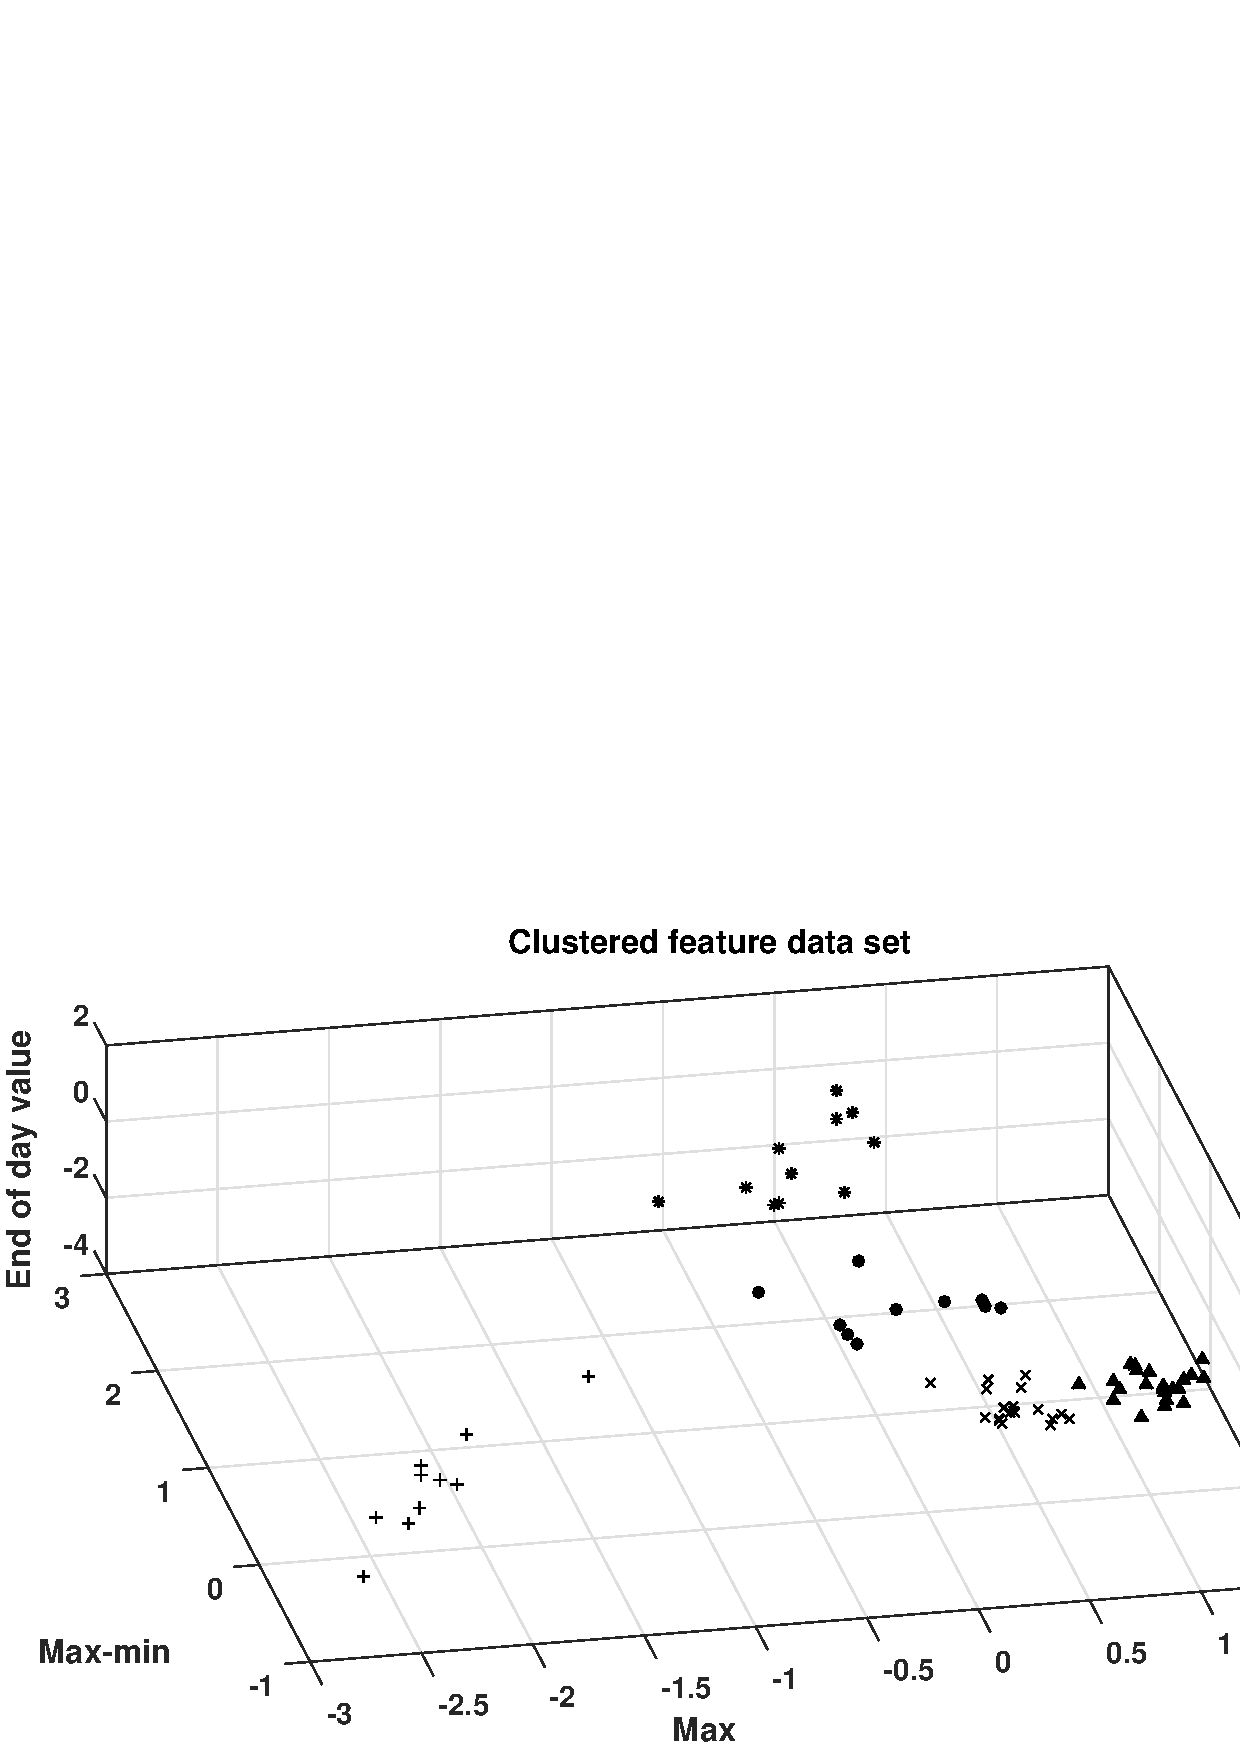
\includegraphics[width = 0.9\textwidth]{Wykresy/clusteredbw.png}
\caption{Clustering results in feature space (values normalized). Clusters represent Sundays (1), Mondays (2), Saturdays (3), other days in good condition (4), and other days in bad condition (5).}
\label{fig: clusteredbw}
\vspace{-15pt}
\end{figure}

All of those classes are important to be detected and identified. Mondays, Saturdays and Sundays reveal very outlying behavior, hence they are not informative and are detected only to be eliminated from further analysis. On the other hand, theoretically all days of the week could be divided into classes of good and bad conditions, but it would require more data. Greater amount of data might cause points in feature space to fill empty spaces within the clusters. Because of that, point clouds would be denser and more consistent. It would allow the Silhouette criterion to estimate larger optimal cluster amount, which then could possibly lead to  distinction between good and bad condition on Mondays, Saturdays and Sundays.
This outcome is impossible to obtain with the currently possessed amount of data, even if we force larger amount of clusters, because classification algorithm cannot properly construct clusters with this little amount of points in feature space. Fig. \ref{fig: cplotbw} presents the results in time domain. Algorithm assigned particular days to correct classes.
\begin{figure}[ht!]
\vspace{-10pt}
\centering
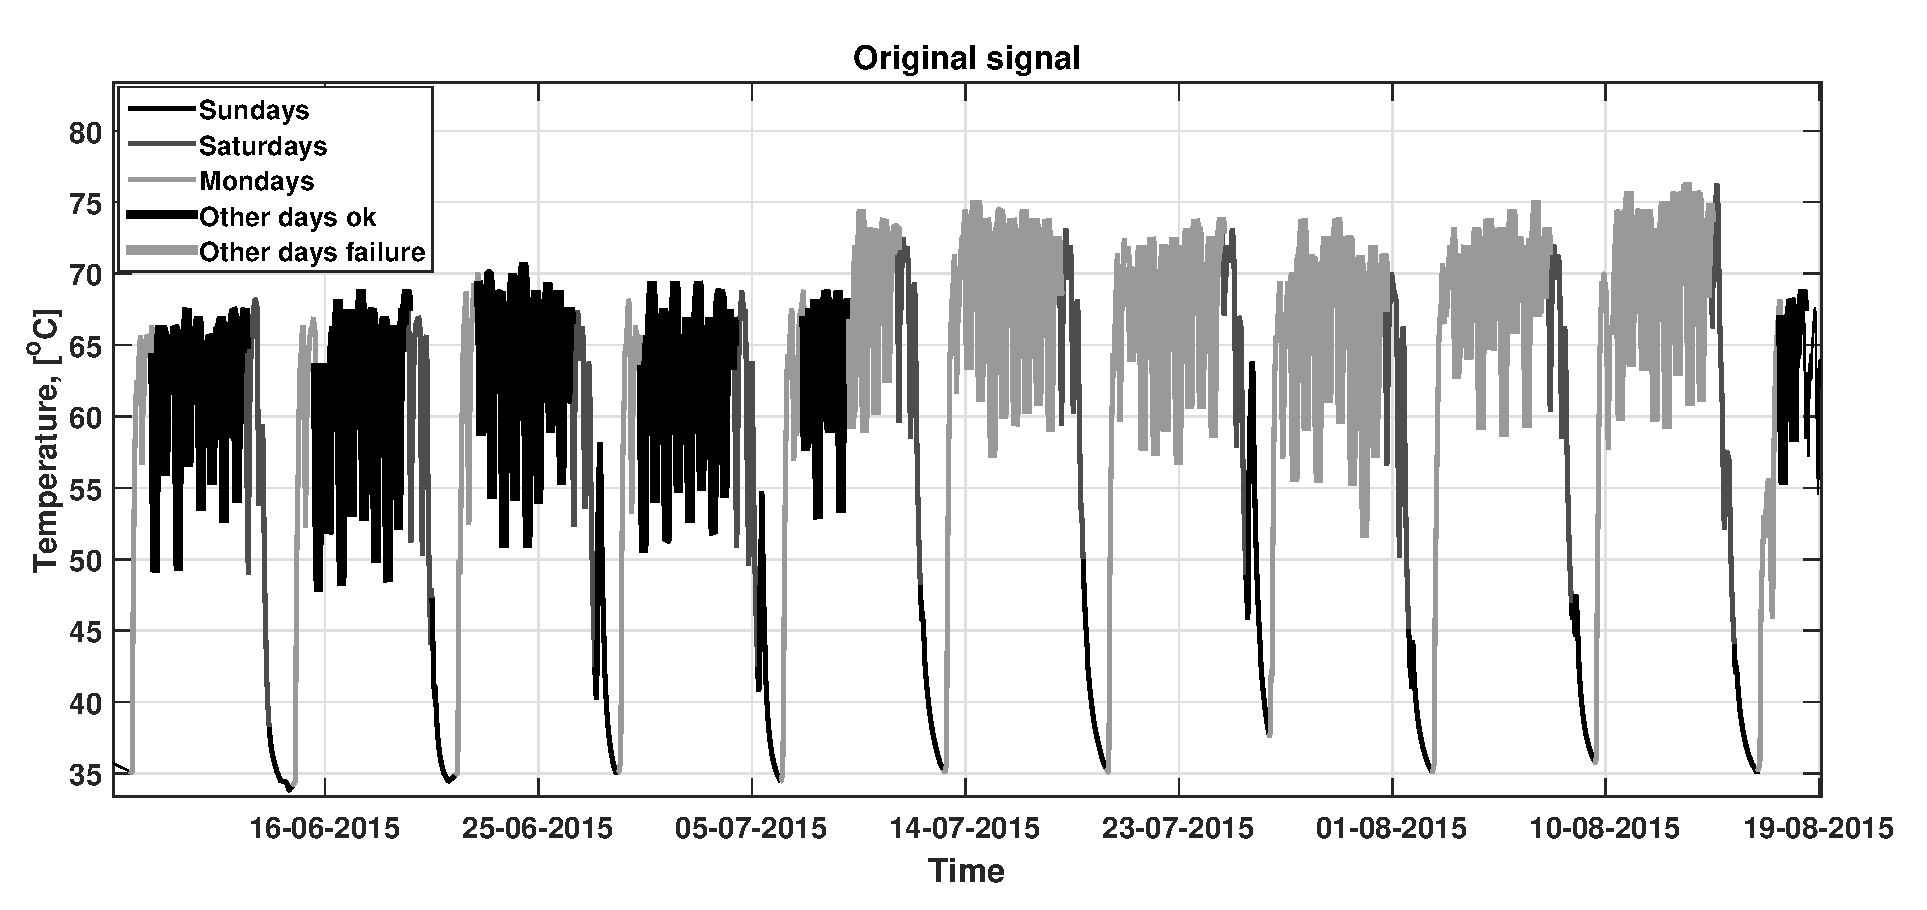
\includegraphics[width = \textwidth]{Wykresy/cplotbw.eps}
\caption{Clustering results in time domain.}
\label{fig: cplotbw}
\vspace{-35pt}
\end{figure}
\section{Conclusions}
In this paper we have presented the application of unsupervised learning method used for data classification in order to detect anomalies in diagnostic temperature signal from heavy duty gearbox used in underground mining industry. The methodology is based on Expectation - Maximization algorithm for Gaussian mixture model estimation, and parameterization with simple statistics. Introduced technique applied to real data gives much better and more reliable results than direct one-dimensional time series analysis. Obtained results allow to detect unusual behavior of the gearbox.
\vspace{-15pt}
\section{Acknowledgments}
This work is supported by the Framework Programme for Research and Innovation
Horizon 2020 under grant agreement no. 636834 (DISIRE -Integrated Process Control
based on Distributed In-Situ Sensors into Raw Material and Energy Feedstock)
\vspace{-15pt}
 \begin{thebibliography}{}
\bibitem{Astolfi2014} Astolfi D., Castellani F., Terzi L., \emph{Fault prevention and diagnosis through SCADA temperature data analysis of an onshore wind farm}, 2014, Diagnostyka Vol. 15 No 2, pp. 71-78.
\bibitem{Bartelmus2014} Bartelmus W., \emph{Object and operation supported maintenance for mining equipment},2014, Mining Science. Vol. 21, pp. 7-21.
\bibitem{Blazej2016} Blazej R., Sawicki M., Kirjanow A., Kozlowski T., Konieczna M., \emph{Automatic analysis of themrograms as a means for estimating  technical of a gear system}, 2016, Diagnostyka. Vol. 17 No 2, pp. 43-48.
\bibitem{Bongers2008} Bongers, D.R., Gurgenci, H., \emph{Fault Detection and Identification for Longwall Machinery Using SCADA Data}, 2008, Complex System Maintenance Handbook, Springer Series in Reliability Engineering, pp. 611-641.
\bibitem{c5} Zimroz R., Bartelmus W., Barszcz T., Urbanek J., \emph{Diagnostics of bearings in presence of strong operating conditions non-stationarity-a procedure of load-dependent features processing with application to wind turbine bearings}, 2014, Mechanical Systems and Signal Processing 46 (1), 16-27.
\bibitem{Dempster} Dempster A.P., Laird N.M., Rubin D.B., \emph{Maximum Likelihood from Incomplete Data via the EM Algorithm}, 1977,  Journal of the Royal Statistical Society, Series B 39 (1), pp. 1-38. JSTOR 2984875. MR 0501537.
\bibitem{Hastie} Hastie T.,  Tibshirani R., Friedman J., \emph{The EM algorithm. The Elements of Statistical Learning}, 2001,  New York: Springer, 236-243. ISBN 0-387-95284-5.
\bibitem{Jonak2006}  Jonak J., Gajewski J.,\emph{Operating diagnostics and monitoring issues of selected mining belt conveyers}, 2006 Maintenance and Reliability Vol. 4 No 32, pp. 74-78.
\bibitem{Kaufman} Kaufman L., Rouseeuw P.J., \emph{Finding Groups in Data: An Introduction to Cluster Analysis}, 1990, NJ: John Wiley \& Sons, Inc.
\bibitem{Krol2016} Krol R., Kisielewski W., Kaszuba D., Gladysiewicz L., \emph{Testing belt conveyor resistance to motion in underground mine conditions}, 2016, International Journal of Mining, Reclamation and Environment, http://dx.doi.org/10.1080/17480930.2016.1187967.
\bibitem{Obuchowski} Kruczek P., Obuchowski J., Zimroz R.,  Wy{\l}oma{\'n}ska, \emph{Belt conveyor diagnostics - damage detection based on multivariate data analysis}, 2016, Proceedings of 16th SGEM International Multidisciplinary Scientific GeoConferences. pp. 99-106, doi:10.5593/sgem2016B12.
\bibitem{Neal} Neal R., Hinton G.,  Jordan M.I., \emph{A view of the EM algorithm that justifies incremental, sparse, and other variants}, Learning in Graphical Models (Cambridge, MA: MIT Press) 1999, pp. 355-368. ISBN 0-262-60032-3. Retrieved 2009-03-22.
\bibitem{Rouseeuw} Rouseeuw  P.J., \emph{Silhouettes: a graphical aid to the interpretation and validation of cluster analysis}, 1987,  Journal of Computational and Applied Mathematics. Vol. 20 No 1, pp. 53-65.
\bibitem{Sawicki} Sawicki M., Zimroz R., Wy{\l}oma{\'n}ska, Obuchowski J., Stefaniak P., {\.Z}ak G.,  \emph{An Automatic Procedure for Multidimensional Temperature Signal Analysis of a SCADA System with Application to Belt Conveyor Components}, Procedia Earth and Planetary Science 15, 2015, pp. 781-790.
\bibitem{Stefaniak2015} Stefaniak  P.,  Wylomanska  A.,  Obuchowski  J.,  Zimroz  R., \emph{Procedures  for  decision  thresholds  finding  in  maintenance management  of  belt  conveyor  system  -  statistical  modeling  of  diagnostic  data}, 2015, Proceedings of the 12th International Symposium Continuous Surface Mining - Aachen 2014. Springer, pp. 391-402.
\bibitem{Stefaniak2012} Stefaniak P., Zimroz R., Krol R., Gorniak-Zimroz J., Bartelmus W., Hardygora M., \emph{Some remarks on using condition monitoring for spatially distributed mechanical system belt conveyor network in underground mine - A Case Study}, 2012, Condition Monitoring of Machinery in Non-Stationary Operations. Springer, pp. 497-507, doi:10.1007/978-3-642-28768-8\_51.
\bibitem{Sundberg} Sundberg R., \emph{Maximum likelihood theory for incomplete data from an exponential family}, 1974, Scandinavian Journal of Statistics 1 (2), pp. 49-58. JSTOR 4615553. MR 381110.
%% do poprawy nota biograficznma
\bibitem{Wodecki} Wodecki J., Stefaniak P., Sawicki M., Zimroz R., \emph{Application of Independent Component Analysis in temperature data analysis for gearbox fault detection}, submitted to Applied Condition Monitoring, Springer, 2016
\bibitem{Zhang2010} Zhang, S., \& Xia, X., \emph{Optimal control of operation efficiency of belt conveyor systems}, 2010, Applied Energy. Vol. 87 No 6, pp. 1929-1937.
\end{thebibliography}
\end{document}
% end of file template.tex
